\chapter{Regularization}


\section{Overfitting}
\begin{itemize}
    \item The hypothesis in Figure \ref{fig:overfitting} are:
        \begin{itemize}
            \item $h(x) = \theta_0 + \theta_1x \Rightarrow$ underfitting
            \item $h(x) = \theta_0 + \theta_1x + \theta_2x^2$
            \item $h(x) = \theta_0 + \theta_1x + \theta_2x^2 + \theta_3x^3 + \theta_4x^4 \Rightarrow$ overfitting
        \end{itemize}
    \begin{figure}[!htbp]\label{fig:overfitting}
        \centering
        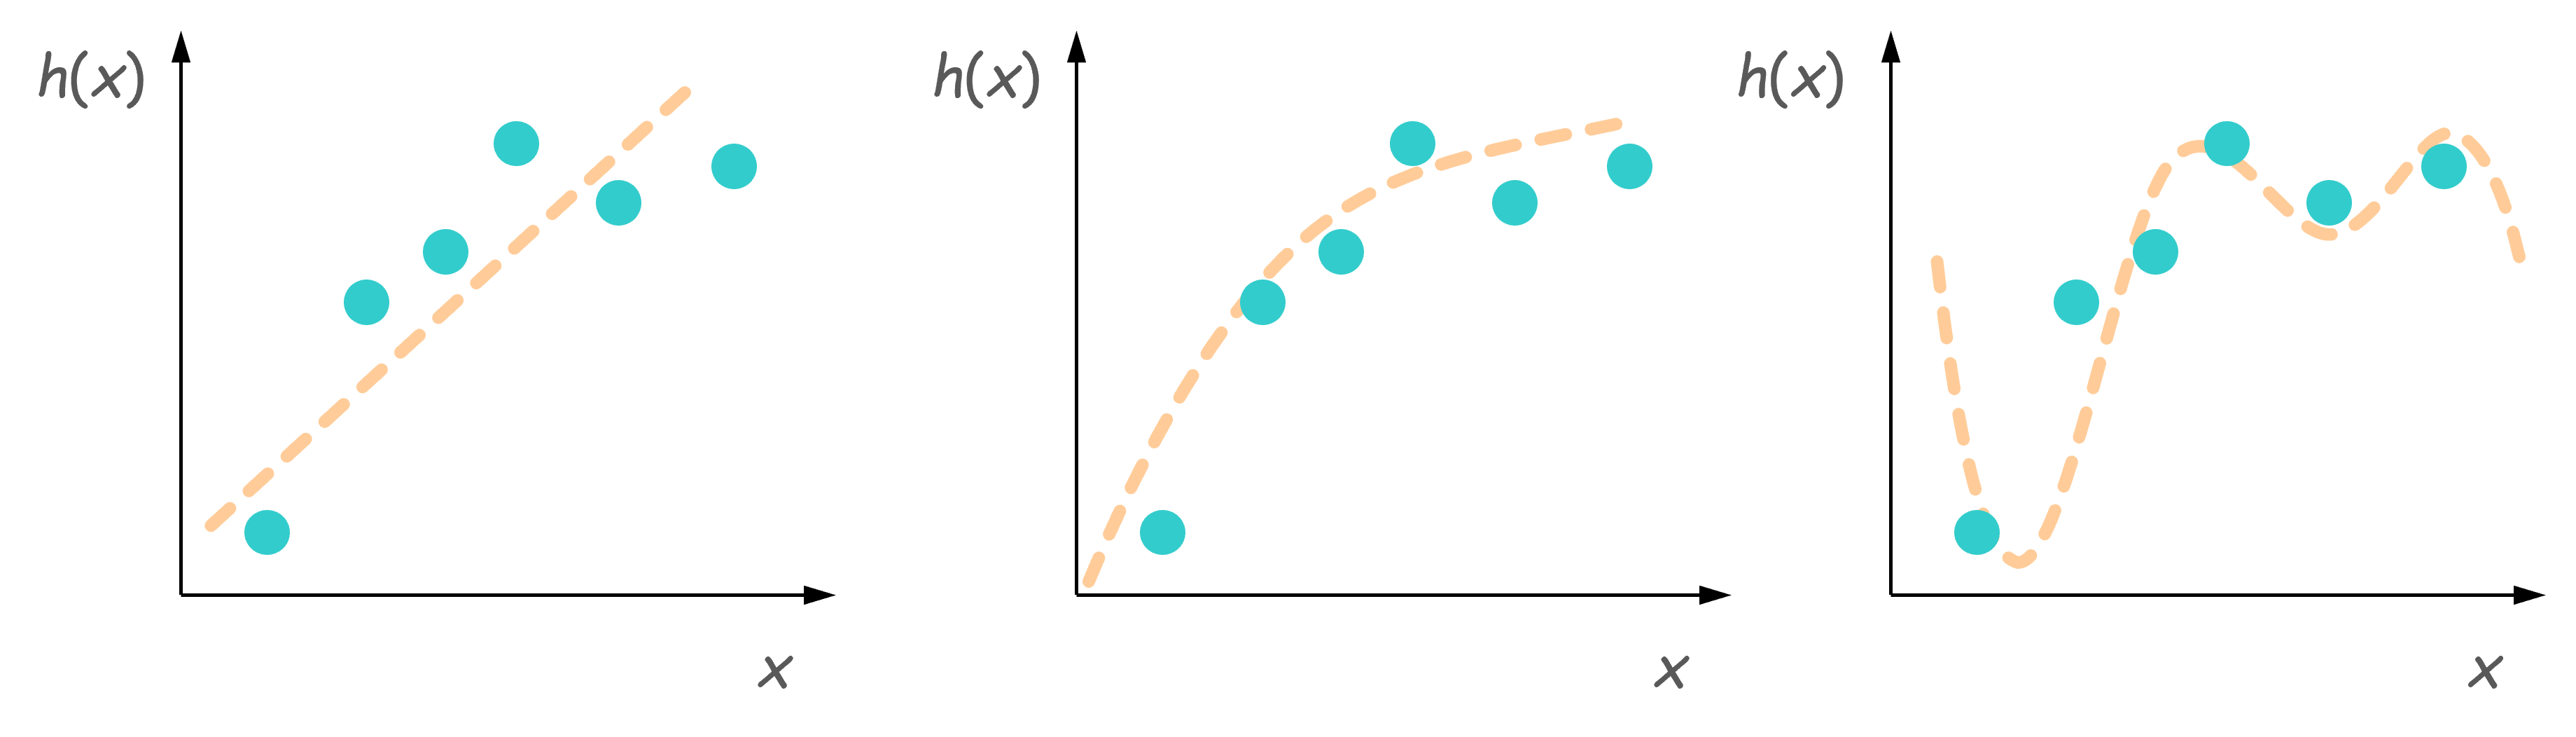
\includegraphics[width=5.4in]{./images/overfitting.png}
        \caption{Three different regression models}
    \end{figure}
    Two main options to address these issue, \textbf{reducing features} and \textbf{regularization}.
    
    \item \textbf{Reduce the number of features}
        \begin{itemize}
            \item Manually select
            \item Use a model selection algorithm
        \end{itemize}
    \item \textbf{Regularization}
        \begin{itemize}
            \item Keep all the features, but reduce the magnitude of parameters $\theta_j$
            \item Works well when slightly features are useful.
        \end{itemize}
\end{itemize}


\section{Regularized Linear Regression}
\begin{itemize}
    \item The intuition of regularization is shown as \ref{fig:intuitionRegularization}
    \begin{figure}[H]\label{fig:intuitionRegularization}
        \centering
        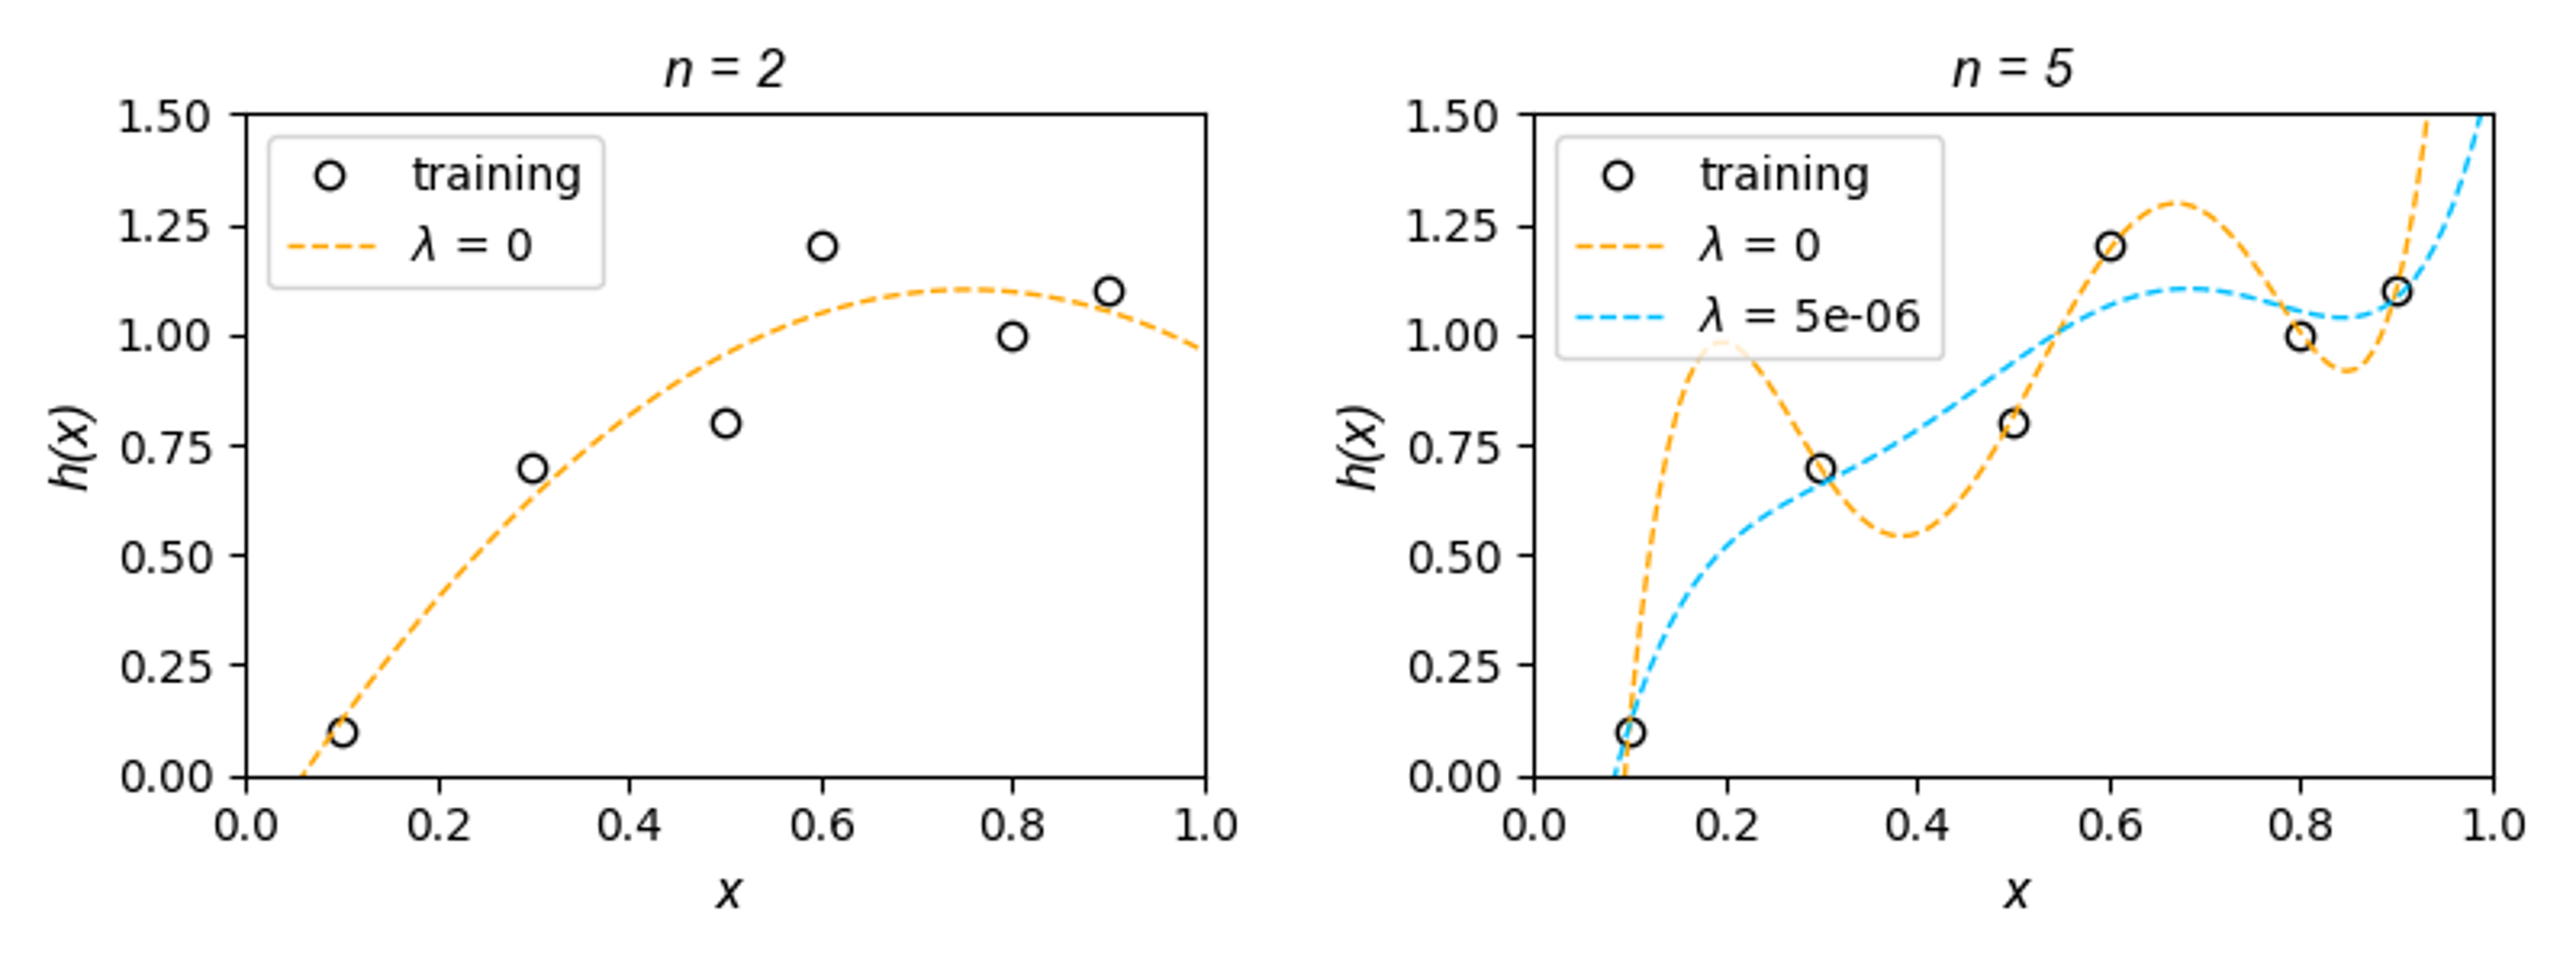
\includegraphics[width=5.4in]{./images/intuitionRegularization.png}
        \caption{The intuition of regularization}
    \end{figure}
    
    \item A regularization term (or regularizer) $\sum_{j=1}^{n}{\theta_j^2}$ is added to the cost function to impose a penalty on the complexity of $h^{(i)}$.
    \begin{equation}\label{eqn:regularCostLinear}
        J(\theta) = \frac{1}{2m} \left[ \sum_{i=1}^{m} { (h^{(i)} - y^{(i)})^2} + \lambda \sum_{j=1}^{n}{\theta_j^2} \right]
    \end{equation}
    The $\mathbf{\lambda}$ is the regularization parameter which controls the importance of the regularization term.
    To reduce the function variety, only the higher-order terms would be penalized, so $\theta_0$ is excluded from the regularization term.

    \item The way to choose the parameters is to find \begin{equation} \min_{\theta}{J\left(\theta\right)} \end{equation}
    Because the regularization term is add to the cost function, the minimization process would not find out the optimum which make $h^{(i)}$ closest to $y^{(i)}$.
    The errors between each $h^{(i)}$ and $y^{(i)}$ would be bigger, so the shape of function would not be too \emph{overfitting}.

    \item To prevent penalize $\theta_0$, it is separated out from the rest of parameters of \textbf{gradient descent} function. 
    \begin{equation}
        \left\{
        \begin{aligned}
            \theta_0 &\coloneqq \theta_0 - \frac{\alpha}{m} \sum_{i=1}^{m} {\left(h^{(i)} - y^{(i)}\right)x_0^{(i)}}\\
            \theta_j &\coloneqq \theta_j - \frac{\alpha}{m} \sum_{i=1}^{m} \left[ {\left( h^{(i)} - y^{(i)}\right)x_j^{(i)} + \lambda\theta_j} \right]\\
        \end{aligned}
        \right.
    \end{equation}
    for $j = 1, \dots, n$ and $j \neq 0$. The vectorized implementation would be
    \begin{equation}
        \mathbf{\theta} \coloneqq \mathbf{\theta} - \frac{\alpha}{m} \left[ \mathbf{X}^T \left(\mathbf{h} - \mathbf{y}\right) + \lambda\mathbf{L}\mathbf{\theta} \right]
    \end{equation}
    where
    \begin{equation}
        \mathbf{L} = 
        \left[
        \begin{matrix}
            0      &        &        &        &       \\
                   & 1      &        &        &       \\
                   &        & 1      &        &       \\
                   &        &        & \ddots &       \\
                   &        &        &        & 1     \\
        \end{matrix}
        \right]
    \end{equation}
    \item And the regularized \textbf{normal equation} becomes
    \begin{equation}\label{eqn:normalRegularized}
        \begin{split}
            \mathbf{\theta} = \left(\mathbf{X}^T\mathbf{X} + \lambda \mathbf{L}\right)^{-1}\mathbf{X}^T\mathbf{y}\\
        \end{split}
    \end{equation}

    Recall that if $m<n$, then $\mathbf{X}^T\mathbf{X}$ is non-invertible. However, when we add the term $\lambda\mathbf{L}$, then $\mathbf{X}^T\mathbf{X} + \lambda\mathbf{L}$ becomes invertible.
    \begin{proof}
        \begin{equation}
            \begin{split}
                J(\mathbf{\theta}) &= \frac{1}{2m} \left[ \left(\mathbf{X}\mathbf{\theta}-\mathbf{y}\right)^{T}\left(\mathbf{X}\mathbf{\theta}-\mathbf{y}\right) + \lambda\mathbf{\theta}^T\mathbf{L}\mathbf{\theta} \right]\\
                                   &= \frac{1}{2m} \left[ \mathbf{\theta}^{T}\mathbf{X}^{T}\mathbf{X}\mathbf{\theta} - 2\left(\mathbf{X}\mathbf{\theta}\right)^{T}\mathbf{y} + \mathbf{y}^{T}\mathbf{y} + \lambda\mathbf{\theta}^T\mathbf{L}\mathbf{\theta} \right]
            \end{split}
        \end{equation}

        Derive by $\mathbf{\theta}$ and compare to 0, $\frac{\partial J}{\partial\mathbf{\theta}} = 0$
        \begin{equation}
            \begin{split}
                2\mathbf{X}^T\mathbf{X}\mathbf{\theta} - 2\mathbf{X}^T\mathbf{y} + 2\lambda\mathbf{L}\mathbf{\theta}= 0\\
                (\mathbf{X}^T\mathbf{X} + \lambda\mathbf{L})\mathbf{\theta} = \mathbf{X}^T\mathbf{y}\\
                \mathbf{\theta} = \left(\mathbf{X}^T\mathbf{X} + \lambda\mathbf{L}\right)^{-1}\mathbf{X}^T\mathbf{y}
            \end{split}
        \end{equation}
    \end{proof}
\end{itemize}


\section{Regularized Logistic Regression}
\begin{itemize}
    \item The way to regularize a logistic regression is similar to linear regression.
    \begin{figure}[H]\label{fig:logisticFit}
        \centering
        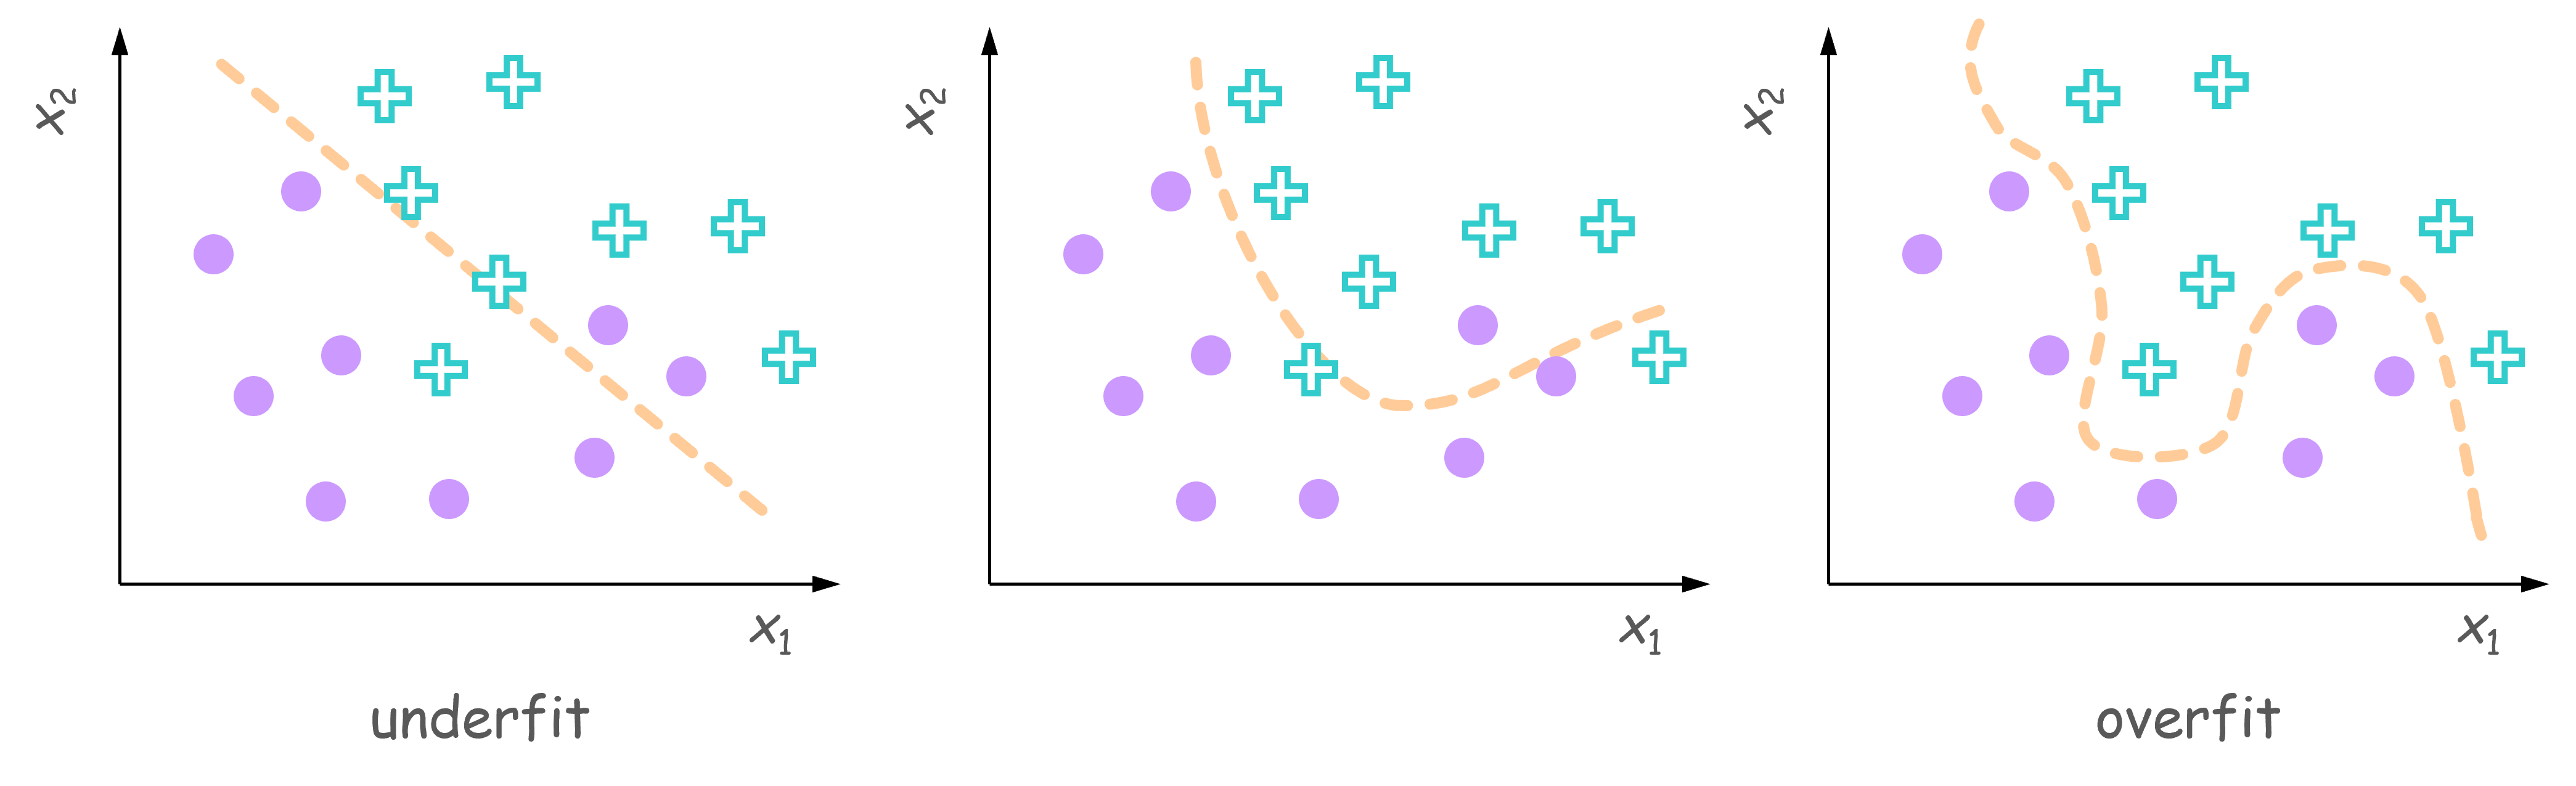
\includegraphics[width=5.4in]{./images/logisticFit.png}
        \caption{Three different regression models}
    \end{figure}
    
    \item Define the cost function
    \begin{equation}
        J(\mathbf{\theta}) = \frac{-1}{m}\sum_{i=1}^{m}{\left[y^{(i)} \log{(h^{(i)})} + (1-y^{(i)}) \log{(1-h^{(i)})} \right]} + \frac{\lambda}{2m}\sum_{j=1}^{n}{\theta_j^2}
    \end{equation}
    The regularization term is added and it is the same as which in (\ref{eqn:regularCostLinear}).
    
    \item Gradient descent
    \begin{equation}
        \left\{
        \begin{aligned}
            \theta_0 &\coloneqq \theta_0 - \frac{\alpha}{m} \sum_{i=1}^{m} {\left(h^{(i)} - y^{(i)}\right)x_0^{(i)}}\\
            \theta_j &\coloneqq \theta_j - \frac{\alpha}{m} \sum_{i=1}^{m} \left[ {\left( h^{(i)} - y^{(i)}\right)x_j^{(i)} + \lambda\theta_j} \right]\\
        \end{aligned}
        \right.    
    \end{equation}
    for $j = 1, \dots, n$ and $j \neq 0$. The vectorized implementation would be
    \begin{equation}
        \mathbf{\theta} \coloneqq \mathbf{\theta} - \frac{\alpha}{m} \left[ \mathbf{X}^T \left(\mathbf{h} - \mathbf{y}\right) + \lambda\mathbf{L}\mathbf{\theta} \right]
    \end{equation}
\end{itemize}
    